
\title{Лекция 1\\Основные положения семантической технологии проектирования интеллектуальных компьютерных систем нового поколения \vspace{-2em}} 
\author[]{Шункевич Д.В.}
\institute[]{Белорусский государственный университет информатики и радиоэлектроники}

\begin{frame}
	\titlepage
\end{frame}

\begin{frame}{\\Содержание лекции}
	\vspace{10mm}
	\topline
	\justifying
	\begin{itemize}
		\item интеллектуальная система, комплексная задача, гибридная интеллектуальная система
		\item основные положения семантической технологии проектирования интеллектуальных компьютерных систем нового поколения
		\item основные компоненты указанной технологии
		\item информационная конструкция, формальный язык, знак, синтаксис, семантика
		\item семантической память
	\end{itemize}

\end{frame}

\begin{frame}{\\*}
	\begin{SCn}
		\scnheader{интеллектуальная система} 
		\scnidtf{система, которая может легко \underline{научиться решать} новые задачи} 
		\scnrelfrom{отличительный признак}{обучаемость}
		\begin{scnrelfromset}{важно отличать}
			\scnitem {способность обучаться более качественному решению задач определенного ограниченного класса (как это делают нейросетевые модели)}
			\scnitem {способность переходить от решения задач одного класса к решению задач другого класса (с ограничениями или без них)}
		\end{scnrelfromset}
	\end{SCn}
\end{frame}

\begin{frame}{\\*}
	\begin{SCn}
		\scnheader{комплексная задача}
		\scnidtf{задача, для решения которой необходимо использовать различные виды заний и различные модели решения задач}
		\begin{scnrelfrom}{примечание}
	 		{Для комплексных задач невозможно заранее сказать, какой набор моделей потребуется для решения}
		\end{scnrelfrom}
		\vspace{5mm}
		Примеры комплексных задач:
		\begin{itemize}
			\item понимание естественных языков, изображений, речевых сообщений 
			\item планирование поведения интеллектуальных роботов.
		\end{itemize}
	\end{SCn}
\end{frame}

\begin{frame}{\\*}
	\begin{SCn}
		\scnheader{гибридная интеллектуальная система} 
		\scnidtf{интеллектуальная система, интегрирующая различные виды знаний и различные модели решения задач}
		\begin{scnrelfrom}{примечание}
			{Именно ГИС способны решать комплексные задачи}
		\end{scnrelfrom}
		\begin{scnrelfromset}{недостатки современных ГИС}
			\scnitem{монолитность}
			\scnitem{ориентированность на решение конкретной задачи, а не различных классов задач}
			\scnitem{требование колоссальных ресурсов для разработки систем}
			\scnitem{невозможность повторного использования компонентов систем для решения других задач (необходимо все делать заново)}
		\end{scnrelfromset}
	\end{SCn}
\end{frame}

\begin{frame}{\\*}
	\begin{SCn}
		\scnheader{OSTIS}
		\scnidtf{Open Semantic Technology for Intelligent Systems}
		\scnidtf{открытая комплексная технология проектирования совместимых интеллектуальных систем}
			\vspace{3mm}
		\begin{scnrelfromset}{основные положения}
			\scnitem {база знаний OSTIS может описывать любой вид знаний}
			\scnitem {решатель задач OSTIS основан на многоагентном подходе и позволяет легко комбинировать любые модели решения задач}
			\scnitem {интерфейс ostis-системы представляет собой подсистему со своей БЗ и решателем задач (также может быть описан с помощью SC-кода)}
			\scnitem {использование универсального способа представления (кодирования) информации, получившего название SC-код }
	
		\end{scnrelfromset}
	\end{SCn}
\end{frame}

\begin{frame}{\\*}	
	\begin{SCn}
	\scnheader{OSTIS}
	\begin{scnrelfromset}{достоинтсва}
		\scnitem {унифицированность представления (любая информация представляется одинаково)}
		\scnitem {удобство машинной обработки и восприятия человеком}
		\scnitem {любые знания и модели решения задач легко интегрируются в ostis-систему (по принципу plug \& play) и её всегда можно переобучить}
		\scnitem {универсальность и совместимость компонентов (повторное использование позволяет сократить время разработки новых компонентов на 40-60\%)}
		\scnitem {система описывается с помощью SC-кода, поэтому она может анализировать себя, искать в себе ошибки и оптимизировать собственную работу (рефлексивность)}
		\end{scnrelfromset}
	\end{SCn}
\end{frame}

\begin{frame}{\\*}
	\begin{SCn}	
		\scnheader{OSTIS}
		\begin{scnrelfromset}{достоинтсва}
			\scnitem {платформенная независимость (разработка независима от операционной системы и архитектуры компьютера, платформа может быть реализована как в программном варианте, так и в аппаратном)}
			\scnitem {параллельная обработка информации}
			\scnitem {ostis-система может включать в себя компоненты, разработанные на базе OSTIS, а также объединяться с любыми другими системами и интегрировать другие компоненты через специальный протокол обмена информацией (JSON) и/или программный интерфейс (API)}
			\scnitem {производительность ostis-системы не хуже традиционной системы, а иногда может оказаться лучше за счёт параллельной обработки (при переходе на семантические компьютеры производительность будет ещё выше)}
		\end{scnrelfromset}
	\end{SCn}
\end{frame}
  
\begin{frame}{\\*}
	\begin{SCn}	
		\scnheader{OSTIS}
		\begin{scnrelfromset}{важно понимать}
			\scnitem  {OSTIS -- это не конкретная интеллектуальная система, а технология разработки интеллектуальных систем, каждая из которых будет решать задачи определенного класса}
			\scnitem {ключевые преимущества OSTIS заключаются не в новых функциональных возможностях разрабатываемых систем (большинство функций ostis-систем можно реализовать с помощью традиционных средств), а в том, насколько легко модифицировать и развивать разрабатываемые системы, адаптировать их к новым задачам, а также насколько эффективно можно накапливать и использовать полученные компоненты при разработке новых систем, сокращая при этом время и трудоёмкость их разработки}
			\scnitem {OSTIS -- это способ решения проблемы совместимости, одной из важнейших проблем современных технологий}
		\end{scnrelfromset}
	\end{SCn}
\end{frame}	

\begin{frame}{\\Архитектура ostis-системы}
	\vspace{10mm}
	\begin{center} 
		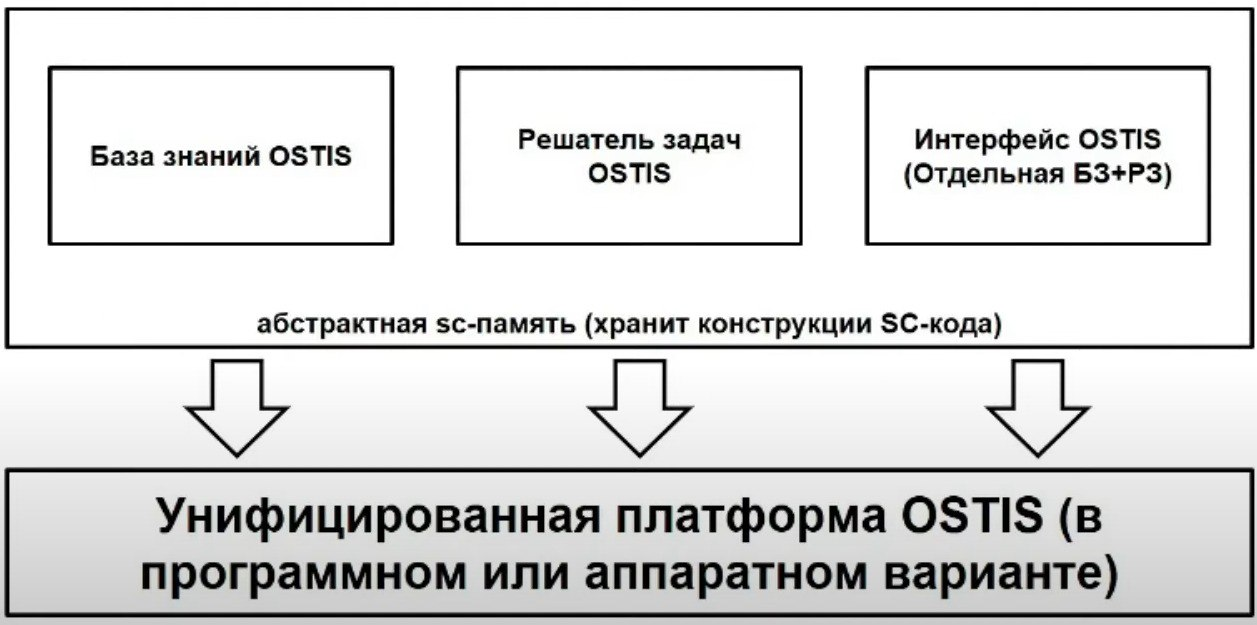
\includegraphics[width=120mm]{./part1/pictures/scheme.jpeg}
	\end{center}
\end{frame}

\begin{frame}{\\*}
	\begin{SCn}	
		\scnheader{база знаний OSTIS}
		\scnidtf{база знаний, описывающая любой вид знаний, при этом её легко дополнять новыми видами знаний}
		\scnheader{решатель задач OSTIS}
		\scnidtf{решатель задач, основанный на многоагентном подходе и позволяющий легко интегрировать и комбинировать любые модели решения задач}
		\scnheader{интерфейс OSTIS}
		\scnidtf{подсистема со своей базой знаний и решателем задач (т.е. так же может быть описан с помощью SC-кода)}
	\end{SCn}
\end{frame}

\begin{frame}{\\*}
	\begin{SCn}
		\scnheader{информационная конструкция}
		\scnidtf{конструкция (структура), содержащая некоторые сведения о некоторых сущностях}	
		\scnidtf{информация}
		\scnrelfrom{примечание}{Информационная конструкция имеет форму представления (текст, звук, изображение), форму структуризации (синтаксис), смысл (денотационную семантику)}
	\end{SCn}
\end{frame}

\begin{frame}{\\*}
	\begin{SCn}
		\scnheader{язык}  
		\scnidtf{множество информационных конструкций, построенных по общим синтаксическим и семантическим правилам}
		\begin{scnrelfromset}{разбиение}
			\scnitem{искуственный (построенный) язык}
			\scnitem{формальный язык}
			\scnitem{естественный язык}
		\end{scnrelfromset}
		\scnheader{формальный язык}  
		\scnidtf{язык, в котором значение каждого слова или знака, правила построения предложений и понимания их смысла однозначны.}
		\scnidtf{множество строк над конечным алфавитом языка}		
	\end{SCn}
\end{frame}

\begin{frame}{\\*}
	\begin{SCn}
		\scnheader{знак}
		\scnidtf{фрагмент информационной конструкции, обладающий свойством, \underline{обозначать} некоторую сущность (объект), которая наряду с другими сущностями описывается указанной информационной конструкцией}
		\scnheader{семиотика}
		\scnidtf{наука о знаках}
		\begin{scnrelfromset}{разбиение}
			\scnitem{синтаксис (изучает правильное построение текста)}
			\scnitem{семантика (изучает значение знаков)}
			\scnitem{прагматика (изучает отношение между знаком и субъектом)}
		\end{scnrelfromset}
	\end{SCn}
\end{frame}

\begin{frame}{\\*}
	\begin{SCn}
		\scnheader{семантическая сеть}
		\scnidtf{граф, вершины которого являются знаками некоторых сущностей, а дуги (ребра) – знаками связей между этими сущностями}
		\scnheader{семантика знака}
		\scnidtf{отношение между знаком и сущностью (значением знака, денотатом), которую он обозначает}
		\begin{center}
			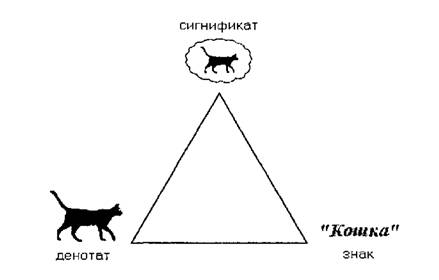
\includegraphics[width=60mm]{./part1/pictures/sc-code-cat.jpg}
		\end{center}
	\end{SCn}
\end{frame}

\begin{frame}{\\*}
	\begin{center}
		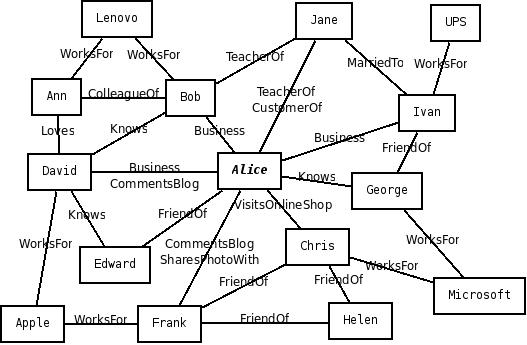
\includegraphics[width=100mm]{./part1/pictures/sc-code-web.jpg}
	\end{center}
\end{frame}

\begin{frame}{\\*}
	\scnheader{синтаксис}
	\scnidtf{наука, изучающая отношения между знаками}
	\scnrelfrom{перевод}{порядок, координация}
	\scnheader{семантика}
	\scnidtf{наука, изучающая отношения между знаками и их значениями}
	\scnrelfrom{перевод}{обозначение, значение}
\end{frame}

\begin{frame}{\\*}
	\begin{SCn}
		\scnheader{семантическая память}
		\scnidtf{графодинамическая (нелинейная) память}
		\scnidtf{смысловая память, обеспечивающая хранение семантических сетей}
		\scnrelfrom{примечание}{изменение семантической памяти происходит не только путем изменения состояния элементов памяти (вершин графа), но также и изменением конфигурации связей между элементами (ребер или дуг графа)}
	\end{SCn}
\end{frame}



